\documentclass{standalone}
\usepackage{tikz}
\usetikzlibrary{patterns, positioning}


\begin{document}
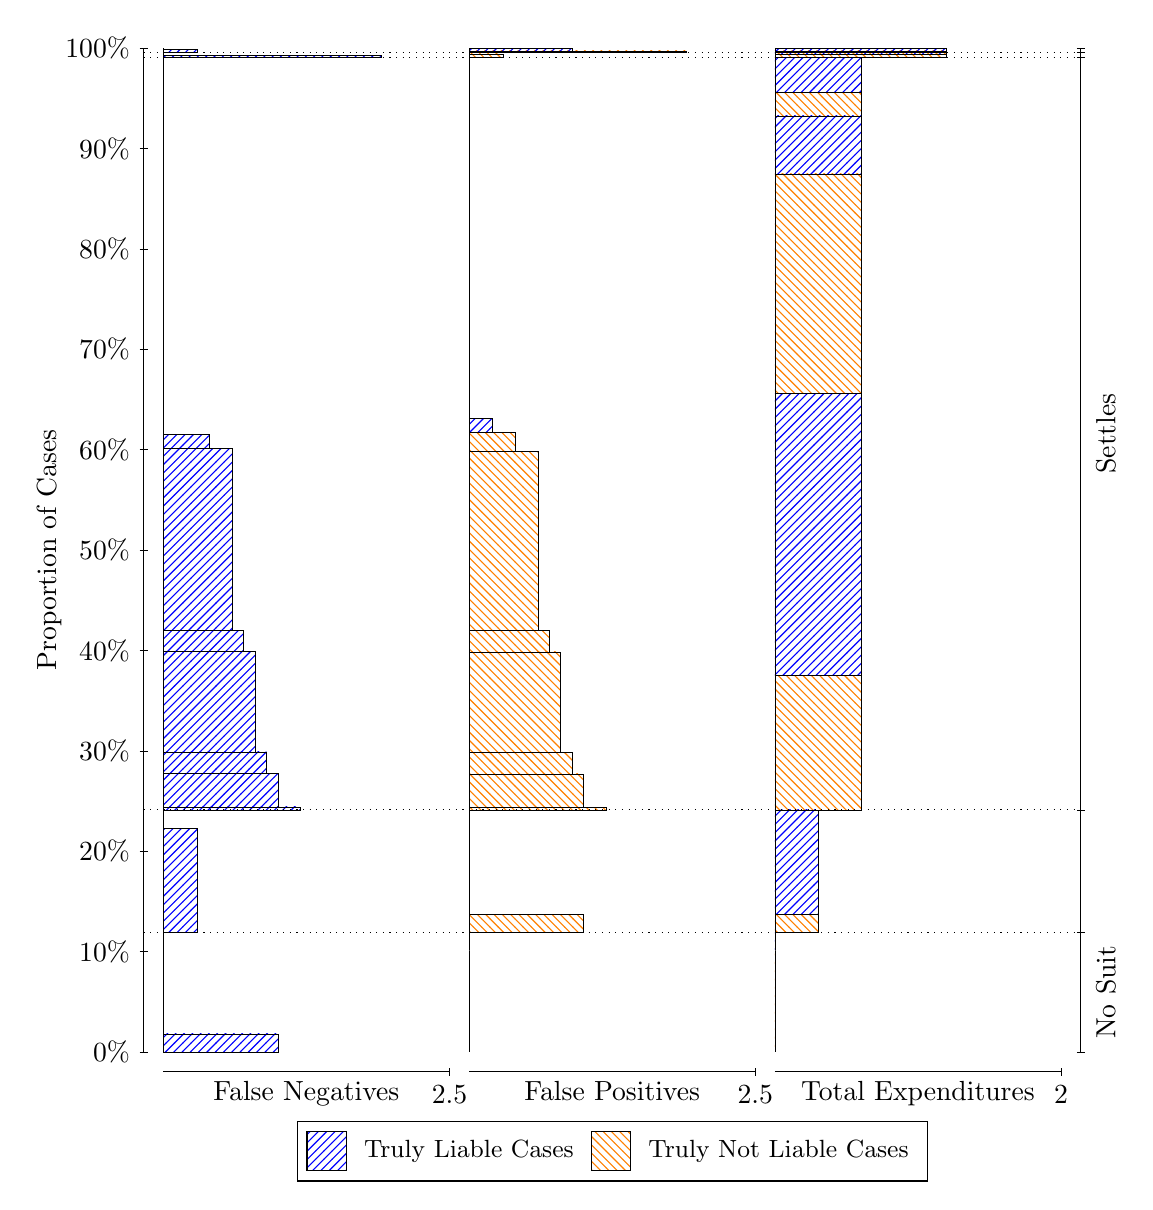
\begin{tikzpicture}
\draw[black, very thin] (1.5,1.75) -- (1.5,14.5);
\node[rotate=90, text=black, anchor=center] at (0.3, 8.125) {Proportion of Cases};
\draw[black, very thin] (1.45,1.75) -- (1.55,1.75);
\node[text=black, anchor=east] at (1.45, 1.75) {0\%};
\draw[black, very thin] (1.45,3.025) -- (1.55,3.025);
\node[text=black, anchor=east] at (1.45, 3.025) {10\%};
\draw[black, very thin] (1.45,4.3) -- (1.55,4.3);
\node[text=black, anchor=east] at (1.45, 4.3) {20\%};
\draw[black, very thin] (1.45,5.575) -- (1.55,5.575);
\node[text=black, anchor=east] at (1.45, 5.575) {30\%};
\draw[black, very thin] (1.45,6.85) -- (1.55,6.85);
\node[text=black, anchor=east] at (1.45, 6.85) {40\%};
\draw[black, very thin] (1.45,8.125) -- (1.55,8.125);
\node[text=black, anchor=east] at (1.45, 8.125) {50\%};
\draw[black, very thin] (1.45,9.4) -- (1.55,9.4);
\node[text=black, anchor=east] at (1.45, 9.4) {60\%};
\draw[black, very thin] (1.45,10.675) -- (1.55,10.675);
\node[text=black, anchor=east] at (1.45, 10.675) {70\%};
\draw[black, very thin] (1.45,11.95) -- (1.55,11.95);
\node[text=black, anchor=east] at (1.45, 11.95) {80\%};
\draw[black, very thin] (1.45,13.225) -- (1.55,13.225);
\node[text=black, anchor=east] at (1.45, 13.225) {90\%};
\draw[black, very thin] (1.45,14.5) -- (1.55,14.5);
\node[text=black, anchor=east] at (1.45, 14.5) {100\%};

\draw[black, very thin] (13.4,1.75) -- (13.4,14.5);
\draw[black, very thin] (13.35,1.75) -- (13.45,1.75);
\node[anchor=west] at (13.35, 1.75) {};
\draw[black, very thin] (13.35,3.2671) -- (13.45,3.2671);
\node[anchor=west] at (13.35, 3.2671) {};
\draw[black, very thin] (13.35,4.8242) -- (13.45,4.8242);
\node[anchor=west] at (13.35, 4.8242) {};
\draw[black, very thin] (13.35,14.385) -- (13.45,14.385);
\node[anchor=west] at (13.35, 14.385) {};
\draw[black, very thin] (13.35,14.444) -- (13.45,14.444);
\node[anchor=west] at (13.35, 14.444) {};
\draw[black, very thin] (13.35,14.5) -- (13.45,14.5);
\node[anchor=west] at (13.35, 14.5) {};

\draw[black, very thin, pattern color=blue, pattern=north east lines] (1.75,1.75) rectangle (3.2033,1.9809);
\draw[black, very thin, pattern color=orange, pattern=north west lines] (1.75,1.9809) rectangle (1.75,3.2671);
\draw[black, very thin, pattern color=blue, pattern=north east lines] (1.75,3.2671) rectangle (2.186,4.5901);
\draw[black, very thin, pattern color=orange, pattern=north west lines] (1.75,4.5901) rectangle (1.75,4.8242);
\draw[black, very thin, pattern color=blue, pattern=north east lines] (1.75,4.8242) rectangle (3.494,4.8615);
\draw[black, very thin, pattern color=blue, pattern=north east lines] (1.75,4.8615) rectangle (3.2033,5.2872);
\draw[black, very thin, pattern color=blue, pattern=north east lines] (1.75,5.2872) rectangle (3.058,5.5599);
\draw[black, very thin, pattern color=blue, pattern=north east lines] (1.75,5.5599) rectangle (2.9127,6.8327);
\draw[black, very thin, pattern color=blue, pattern=north east lines] (1.75,6.8327) rectangle (2.7673,7.1037);
\draw[black, very thin, pattern color=blue, pattern=north east lines] (1.75,7.1037) rectangle (2.622,9.4128);
\draw[black, very thin, pattern color=blue, pattern=north east lines] (1.75,9.4128) rectangle (2.3313,9.5887);
\draw[black, very thin, pattern color=orange, pattern=north west lines] (1.75,9.5887) rectangle (1.75,14.385);
\draw[black, very thin, pattern color=blue, pattern=north east lines] (1.75,14.385) rectangle (4.5113,14.404);
\draw[black, very thin, pattern color=orange, pattern=north west lines] (1.75,14.404) rectangle (1.75,14.444);
\draw[black, very thin, pattern color=blue, pattern=north east lines] (1.75,14.444) rectangle (2.186,14.481);
\draw[black, very thin, pattern color=orange, pattern=north west lines] (1.75,14.481) rectangle (1.75,14.5);
\draw[black, very thin, pattern color=orange, pattern=north west lines] (5.6333,1.75) rectangle (5.6333,3.0362);
\draw[black, very thin, pattern color=blue, pattern=north east lines] (5.6333,3.0362) rectangle (5.6333,3.2671);
\draw[black, very thin, pattern color=orange, pattern=north west lines] (5.6333,3.2671) rectangle (7.0867,3.5012);
\draw[black, very thin, pattern color=blue, pattern=north east lines] (5.6333,3.5012) rectangle (5.6333,4.8242);
\draw[black, very thin, pattern color=orange, pattern=north west lines] (5.6333,4.8242) rectangle (7.3773,4.8521);
\draw[black, very thin, pattern color=orange, pattern=north west lines] (5.6333,4.8521) rectangle (7.0867,5.2818);
\draw[black, very thin, pattern color=orange, pattern=north west lines] (5.6333,5.2818) rectangle (6.9413,5.5545);
\draw[black, very thin, pattern color=orange, pattern=north west lines] (5.6333,5.5545) rectangle (6.796,6.83);
\draw[black, very thin, pattern color=orange, pattern=north west lines] (5.6333,6.83) rectangle (6.6507,7.1011);
\draw[black, very thin, pattern color=orange, pattern=north west lines] (5.6333,7.1011) rectangle (6.5053,9.3764);
\draw[black, very thin, pattern color=orange, pattern=north west lines] (5.6333,9.3764) rectangle (6.2147,9.6203);
\draw[black, very thin, pattern color=blue, pattern=north east lines] (5.6333,9.6203) rectangle (5.924,9.7962);
\draw[black, very thin, pattern color=blue, pattern=north east lines] (5.6333,9.7962) rectangle (5.6333,14.385);
\draw[black, very thin, pattern color=orange, pattern=north west lines] (5.6333,14.385) rectangle (6.0693,14.425);
\draw[black, very thin, pattern color=blue, pattern=north east lines] (5.6333,14.425) rectangle (5.6333,14.444);
\draw[black, very thin, pattern color=orange, pattern=north west lines] (5.6333,14.444) rectangle (8.3947,14.463);
\draw[black, very thin, pattern color=blue, pattern=north east lines] (5.6333,14.463) rectangle (6.9413,14.5);
\draw[black, very thin, pattern color=orange, pattern=north west lines] (9.5167,1.75) rectangle (9.5167,3.0362);
\draw[black, very thin, pattern color=blue, pattern=north east lines] (9.5167,3.0362) rectangle (9.5167,3.2671);
\draw[black, very thin, pattern color=orange, pattern=north west lines] (9.5167,3.2671) rectangle (10.062,3.5012);
\draw[black, very thin, pattern color=blue, pattern=north east lines] (9.5167,3.5012) rectangle (10.062,4.8242);
\draw[black, very thin, pattern color=orange, pattern=north west lines] (9.5167,4.8242) rectangle (10.607,6.5293);
\draw[black, very thin, pattern color=blue, pattern=north east lines] (9.5167,6.5293) rectangle (10.607,10.111);
\draw[black, very thin, pattern color=orange, pattern=north west lines] (9.5167,10.111) rectangle (10.607,12.901);
\draw[black, very thin, pattern color=blue, pattern=north east lines] (9.5167,12.901) rectangle (10.607,13.637);
\draw[black, very thin, pattern color=orange, pattern=north west lines] (9.5167,13.637) rectangle (10.607,13.938);
\draw[black, very thin, pattern color=blue, pattern=north east lines] (9.5167,13.938) rectangle (10.607,14.385);
\draw[black, very thin, pattern color=orange, pattern=north west lines] (9.5167,14.385) rectangle (11.697,14.425);
\draw[black, very thin, pattern color=blue, pattern=north east lines] (9.5167,14.425) rectangle (11.697,14.444);
\draw[black, very thin, pattern color=orange, pattern=north west lines] (9.5167,14.444) rectangle (11.697,14.463);
\draw[black, very thin, pattern color=blue, pattern=north east lines] (9.5167,14.463) rectangle (11.697,14.5);
\draw[black, dotted] (1.5,3.2671) -- (13.4,3.2671);
\draw[black, dotted] (1.5,4.8242) -- (13.4,4.8242);
\draw[black, dotted] (1.5,14.385) -- (13.4,14.385);
\draw[black, dotted] (1.5,14.444) -- (13.4,14.444);
\draw[black, very thin] (1.75,1.5) -- (5.3833,1.5);
\node[text=black, anchor=north] at (3.5667, 1.5) {False Negatives};
\draw[black, very thin] (5.3833,1.45) -- (5.3833,1.55);
\node[text=black, anchor=north] at (5.3833, 1.45) {2.5};

\draw[black, very thin] (5.6333,1.5) -- (9.2667,1.5);
\node[text=black, anchor=north] at (7.45, 1.5) {False Positives};
\draw[black, very thin] (9.2667,1.45) -- (9.2667,1.55);
\node[text=black, anchor=north] at (9.2667, 1.45) {2.5};

\draw[black, very thin] (9.5167,1.5) -- (13.15,1.5);
\node[text=black, anchor=north] at (11.333, 1.5) {Total Expenditures};
\draw[black, very thin] (13.15,1.45) -- (13.15,1.55);
\node[text=black, anchor=north] at (13.15, 1.45) {2};

\node[text=black, centered, rotate=90] at (13.72, 2.5086) {No Suit};

\node[text=black, centered, rotate=90] at (13.72, 9.6045) {Settles};



\draw (7.449999999999999,1.5) node[draw=none] (baseCoordinate) {};
\begin{scope}[align=center]
        \matrix[scale=0.5, draw=black, below=0.5cm of baseCoordinate, nodes={draw}, column sep=0.1cm]{
            \node[rectangle, draw, minimum width=0.5cm, minimum height=0.5cm, pattern color=blue, pattern=north east lines] {}; &
            \node[draw=none, font=\small, text=black] (B) {Truly Liable Cases}; &
            \node[rectangle, draw, minimum width=0.5cm, minimum height=0.5cm, pattern color=orange, pattern=north west lines] {}; &
            \node[draw=none, font=\small, text=black] (B) {Truly Not Liable Cases}; \\
            };
\end{scope}

\end{tikzpicture}
\end{document}